\section{Approach}
In this section, we present our implementation for injecting faults, as well as analysis for predicting program outcome and fault types.

\subsection{Pipeline}
Figure~\ref{fig:pipeline} shows the general pipeline of our proposed system. For any target application, it is first modified to contain at least one all to initialize fault injection. Then it is compiled in the architecture X86 or ALPHA where GemFI support with the specific libraries. In this work, we choose ALPHA as our test architecture as it is lightweight and have full supports by the fault injector. Afterwards, the generated binary should be moved to the disk image serving as the virtual disk of GemFI. The specific faults are provided by the user in a file at command line. Each line of the input file specifies the attributes of a single fault. We will talk in detail about the fault injection in Section \ref{section:FI}. 

GemFI \cite{parasyris2014gemfi} simulator simulates the execution of the target application until a fault is to be activated. When it is time, the GemFI simulator will modify the state of the hardware e.g. flip the bit or set the value to all 0 according to the fault specification. The output of the program may differ based on whether the faults have been masked or not. These outputs will serve as the labels of our training data. GemFi simulator also generates statistics of a fixed-length microarchitecture event periodically. These raw features will serve as the feature vectors of our training data. We will talk about feature extraction in detail in Section \ref{section:FE}. 

Our feature extraction and labeling module will extracts standardized features from raw features and label them according to the result of the test program. These standardized features will then feed into Machine Learning component and ML algorithms will learn meaningful features from them. We will talk about it in Section \ref{section:ML}

\begin{figure}[t]
\begin{center}
   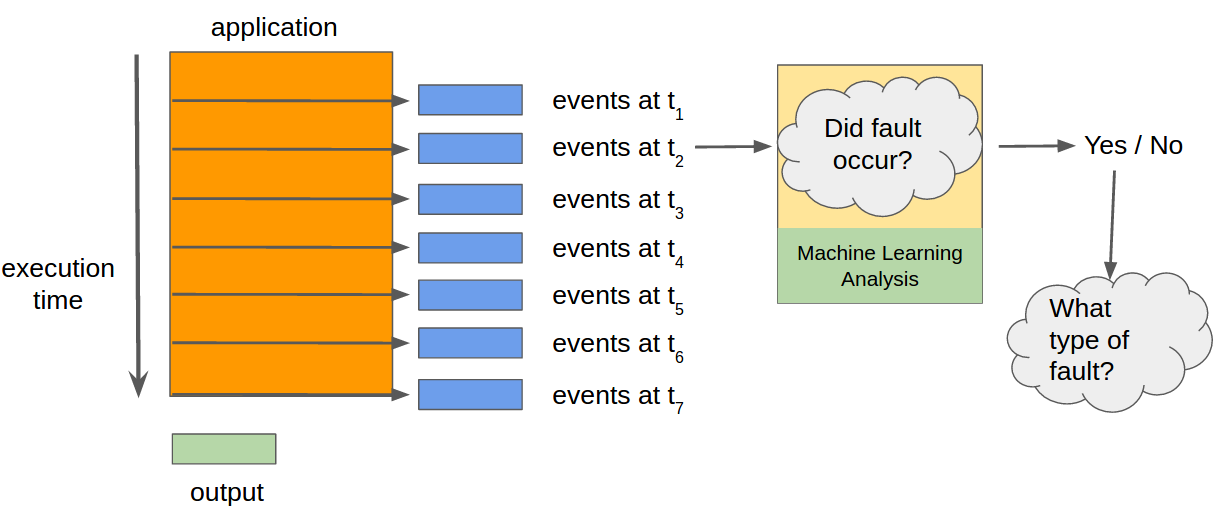
\includegraphics[width=0.95\linewidth]{./figures/teaser.png}
\end{center}
   \caption{\footnotesize Motivation to extract meaningful features}
\label{fig:teaser}
\end{figure}

\begin{figure*}[t]
\begin{center}
   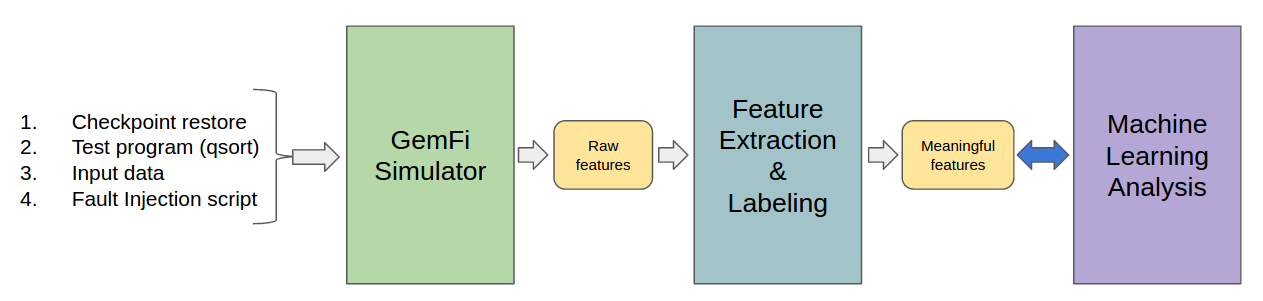
\includegraphics[width=0.95\linewidth]{./figures/pipeline.png}
\end{center}
   \caption{\footnotesize General pipeline of our work. GemFi simulator restores from the checkpoint which saves the warm up stage of the system and takes in test program, input data of the test program and the fault injection script. It then simulates the execution of the program and generates the raw features. Our feature extraction and labeling module will then extract common feature and label each feature vector for binary and multi-class classification. The machine learning algorithms learn models from the features and also output useful features.}
\label{fig:pipeline}
\end{figure*}



\subsection{Fault Injection}\label{section:FI}
The faults are provided by the user through an input file. Each line of the input file specifies the attributes of a single fault. Faults are characterized by four attributes: Location, Thread, Time and Behavior. 
\begin{itemize}
\item Location: Location specifies which microarchitectural modules the fault would be injected into, e.g. registers, the fetched instructions and PC address
\item Thread: Thread offers the flexibility for the user to selectively inject faults
\item Time: Faults are scheduled to the number of instructions already executed, or to the number of elapsed simulation ticks of the targeted thread
\item Behavior: Behavior specifies which operation the fault will corrupt the module. Flipping bits, XORing or setting all bits to 0,1 are some of the operations supported by GemFI
\end{itemize}

An example below shows the a sample input of faults. 
\begin{lstlisting}	
RegisterInjectedFault Inst:17958 Flip:16 
     Threadid:0 system.cpu1 occ:1 int 1
\end{lstlisting}

This example describes a fault that injects into the $16th$ bit of the register R1 of the CPU, when the application fetches $17958th$ instruction after the initiation of fault injection. 

In our work, we focus on four types of faults: \textit{GeneralFetchInjectedFault}, \textit{LoadStoreInjectedFault}, \textit{ExecutionInjectedFault} and \textit{OpCodeInjectedFault}. And we choose the instruction as the criteria for when to inject faults because it is easy for us to know the exact number of instructions for the test application from the output. Flipping bit is the only operation we employ for the fault as this is the most common transient fault which takes place in the real hardware. 



\subsection{Feature Extraction and Labeling}\label{section:FE}
\subsubsection{Feature Extraction}
GemFI generates a \emph{stats} file which contains the statistics for each period of microarchitecture event for different features. However, the number and type of features in each event may vary greatly because of different types of faults, different execution status and different execution results. So in order to get the fixed length of features of each event, we extract all the common features from the \emph{stats} files. 
\subsubsection{Labeling}
There are three kinds of output from the test. The first kind of faults is masked by the hardware and the result is correct. This happens a lot as the operation of flipping the bit is very likely to be masked.The second kind of faults is that the test program encounters the segmentation fault in the middle of the execution. The last kind is that the execution of the program exits normally however the output is not correct. From our trivial observation, among all the faulty execution of the program, the second kind is the one which is most commonly. We will label the first condition as 0 which is the correct output and label the latter two conditions as 1 in binary classification and 1, 2, 3, 4 corresponds to different types of fault in multi-class classification.

\subsection{Checkpoint Restoring}
We also employ checkpoint mechanism to save the simulation time of a test program. For simulating a test program, GemFI first loads the entire linux system in detailed mode and then executes the program. This loading step takes about 5 minutes and usually takes 90\% of the total simulation time. So by creating a checkpoint after the system has been loaded, we can directly simulate the test program next time by restoring this checkpoint. This saves us a lot of time when generating training data by simulating the test programs. 


\subsection{Machine Learning Method}\label{section:ML}
We use the random forest algorithm to predict program outcome and fault type. A random forest is essentially an ensemble of single decision trees \cite{breiman2001random}. It captures different characteristics of the data, with each decision tree representing a model. One particular attractive aspect of random forest is that it allows us to analyze the importance of different features according to the information gain of each feature dimensions. We can use the information gain to rank the importance of each feature and therefore determine which features can be pruned.

%\begin{figure}[t]
%\begin{center}
%   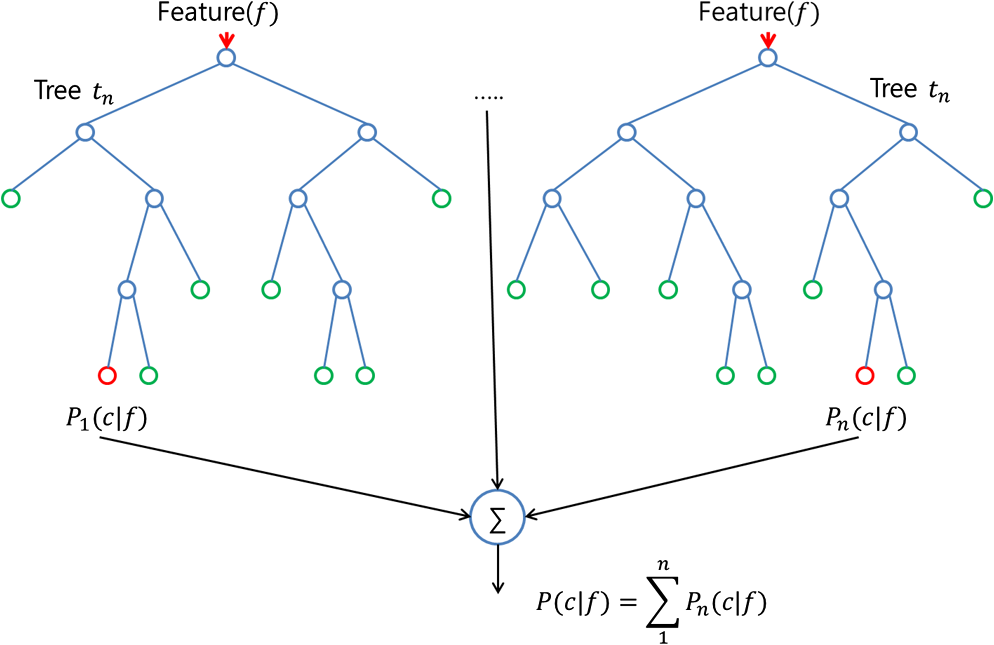
\includegraphics[width=0.95\linewidth]{./figures/rf.png}
%\end{center}
%   \caption{\footnotesize Random forests}
%\label{fig:rf}
%\end{figure}


%\begin{figure}[t]
%\begin{center}
%   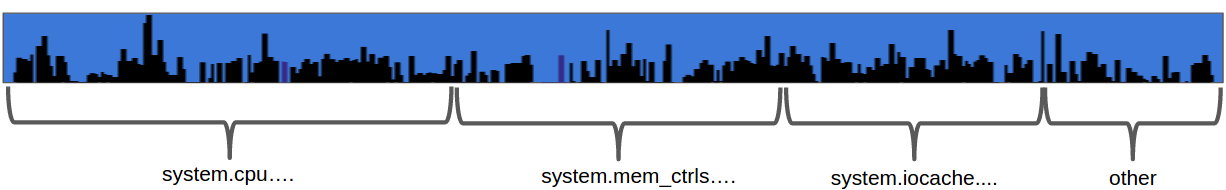
\includegraphics[width=0.95\linewidth]{./figures/feat_dist.png}
%\end{center}
%   \caption{\footnotesize Features in different components of the microachitecture.}
%   \vspace{-0.4cm}
%\label{fig:feat-dist}
%\end{figure}

%Figure~\ref{fig:feat-dist} shows features in different components of the microarchitecture.

We randomly select $60\%$ of instances for training and $40\%$ of instances for testing. Our dataset consists of $98,000$ data instance.
